\documentclass[10pt]{beamer}

\usetheme[progressbar=frametitle]{metropolis}
\usepackage{appendixnumberbeamer}

\usepackage{booktabs}
\usepackage[scale=2]{ccicons}
\usepackage{pgfpages}



\usepackage{pgfplots}
\usepgfplotslibrary{dateplot}

\usepackage{xspace}
%\setbeameroption{show notes on second screen=right} 
%\setbeamertemplate{note page}{\pagecolor{yellow!5}\insertnote}

\pgfdeclareimage[width=\paperwidth]{mybackground}{src/futureits.png}
\defbeamertemplate{description item}{align left}{\insertdescriptionitem\hfill}

\newcommand{\themename}{\textbf{\textsc{metropolis}}\xspace}
\hypersetup{pdfpagemode=FullScreen}




\title{Adaptive Beamforming for future ITS}
\subtitle{A neural network approach to antenna beam steering for mmWave Systems}
\author{Clifford Beta \and \\Anne Okemwa}
 \date{\today}

 \titlegraphic{\hfill
\includegraphics[height=1.5cm]{src/logo.png}}

\begin{document}

\maketitle
    
\begin{frame}{mmWave Communication Potential}
  \begin{itemize}[<+- | alert@+>]
    \item \huge multi-gigabit-per second communication
    \item \huge very low latency
  \end{itemize}
\end{frame}
{
\usebackgroundtemplate{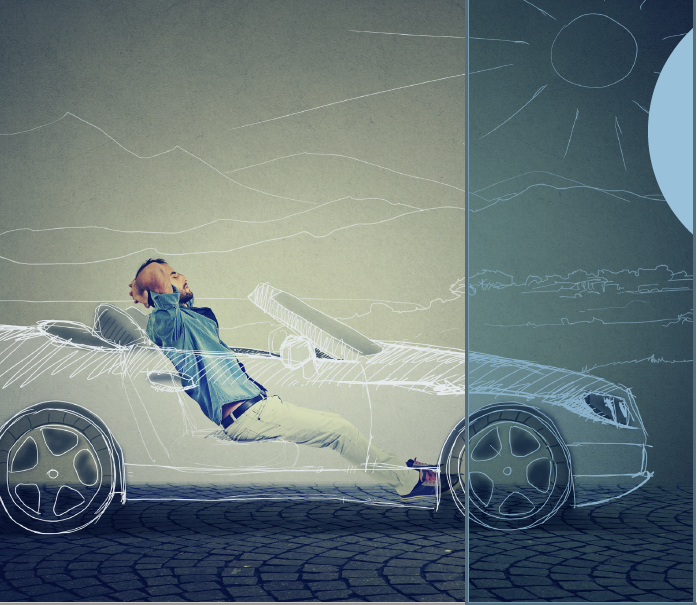
\includegraphics[width=\paperwidth]{src/autonomous.png}}
\begin{frame}{Applications}
  \begin{itemize}[<+- | alert@+>]
    \item \huge Autonomous driving
    \item \huge Immersive gaming
    \item \huge Virtual reality
    \item \huge Augmented reality
  \end{itemize}
\end{frame}
}
\begin{frame}
	%\frametitle{Two Figures aside}
	
	\begin{columns}[b]
		\column{0.0125\textwidth}
		\column{0.4875\textwidth}
		\begin{overlayarea}{\textwidth}{.45\textheight}
 		 \only<1-|handout:0>{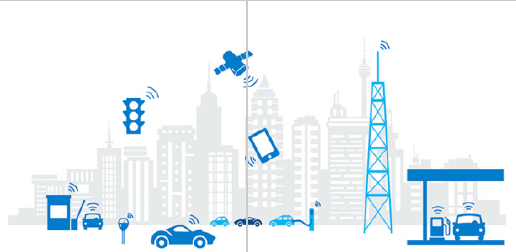
\includegraphics[width=4cm]{src/futureits.png}}
		\end{overlayarea}%
			
		Increased vehicular mobility
		
		\column{0.4875\textwidth}
			\begin{overlayarea}{\textwidth}{.45\textheight}
			  \only<2>{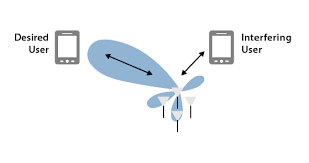
\includegraphics[width=4cm]{src/desired_user.png} }
			\end{overlayarea}
			\par
		Need for constant beam realignment.
		\column{0.0125\textwidth}
		

	\end{columns}
\end{frame}

{
\usebackgroundtemplate{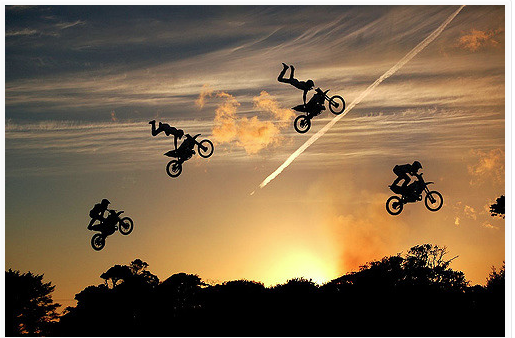
\includegraphics[width=\paperwidth]{src/sequence.png}}
\begin{frame}[fragile]{Model}
 \par
\end{frame}
}

\begin{frame}[fragile]{Neural Network}
  Neural networks have been proven to have the ability to compute any function, even

  \begin{verbatim}   {Sequence prediction problems}\end{verbatim}

  at which \emph{LSTMs} shine \ldots
\end{frame}

\begin{frame}[fragile]{Neuron}
\begin{columns}[b]
		\column{0.0125\textwidth}
		\column{0.4875\textwidth}
		\begin{equation*}   
  		 \Huge\sigma (z) \equiv  \frac{1}{1+ e^ {-z}}
 		 \end{equation*}
		 \\
		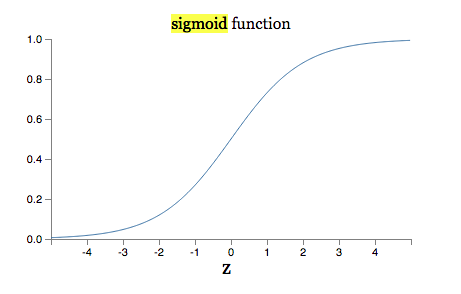
\includegraphics[width=4cm]{src/sigmoidplot.png}
			
		
		
		\column{0.4875\textwidth}
		
		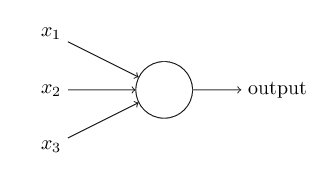
\includegraphics[width=4cm]{src/sigmoid.png} 

			\par
		\column{0.0125\textwidth}
		

	\end{columns}

\end{frame}

\begin{frame}{Neural Network}
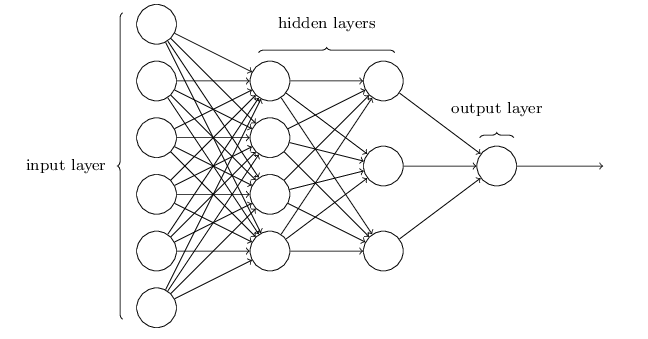
\includegraphics[width=\textwidth]{src/neuralnet.png} 
\begin{itemize}[<+- | alert@+>]
    \item  Feed forward Neural Networks
    \item  Recurrent Neural Networks 
    \begin{itemize}
    \item Long short term memory RNN (LSTM)
    \end{itemize}
  \end{itemize}
\end{frame}

\begin{frame}{Implementation}
\setbeamertemplate{description item}[align left]
	\begin{description}
		\item [Model] LSTM
		\item [Training data] GPS co-ordinates
		\item [Testing]
		\item [Verification]
		\item [Beam forming algorithm] - selection of an appropriate beam forming algorithm
		\item [Deployment]
	\end{description}
\end{frame}

\begin{frame}{Merits}
	\begin{description}
		\item [Higher SNR] 
		%The highly directional transmission improves the link budget, this increasing the range, both open-space and for indoor penetration
		\item [Interference avoidance and rejection] 
		%Beamforming overcomes external and internal (CCI) interference by exploiting the spatial properties of the antennas. Since the interference comes from a certain direction, the 				beamformer can apply a nulling technique ? send a ?null? towards the interferer, canceling it out.
		\item [Higher network efficiency] 
		%By significantly reducing the CCI, beamforming can allow much denser deployments than single antenna systems. Thanks to higher link budget, the likelihood of running high-order 				modulations (64QAM, 16QAM) is much higher even at the edges of the cell. Overall capacity is greatly improved.
	\end{description}
\end{frame}

{\setbeamercolor{palette primary}{fg=black, bg=yellow}
\begin{frame}[standout]
  Questions?
\end{frame}
}

\end{document}
